\chapter{Documentation}\label{ch:documentation}

We have made a literature study containing all the research we have done. 
Below you will find a summary of our most important finds for our project.

\section{Literature Study}

    \subsection{What is LoRa}
        LoRa is a wireless technology that offers long-range, low-power, and secure small packet data transmission for IoT applications. LoRa is based on chirp spread spectrum modulation, which has low power characteristics and can be used for long-range communications. These are some important specifications to know:
        
        \begin{itemize}
            \item standard: 		    LoRaWAN R1.0
            \item frequency band: 	    868MHz (Europe)
            \item data rate: 		    0.3–50 Kb/s
            \item transmission range:	<30 km	
            \item energy consumption:	very low (mA)
        \end{itemize}
    
    \subsection{Project material requirements}
        \subsubsection{Node}
            Every node will contain a LoPy4. This module is responisble for all the calculations and the LoRa communication.
            
            All LoPy4 will have an \href{https://pycom.io/product/lora-868mhz-915mhz-sigfox-antenna-kit/}{antenna} connected to them with the connecter that is part
            of the board.
            
            We will also have to design a LoPy4 shield to be able to connect our microphone pcb
            to receive the data. this shield will also contain a fuse and maybe some LEDs
            to be able to easily see what is going on.
            
            The microphone will be on its own PCB with a JST connector to the LoPy4 shield.
            
            Lastly the node will contain a battery to power everything.
            
        \subsubsection{Gateway}
            Our gateway will exist out of a PyGate shield with a GPY development board and 
            an antenna.
        
    \newpage
    
    \subsection{Hardware}
        \subsubsection{Development board}
            For our development board we have chosen the \href{https://pycom.io/product/lopy4/}{LoPy4}. There are several reasons
            it is better then the competition. Below you find a comparison with the 
            raspberry pi pico.
            
            \begin{table}[h]\centering
            \caption{Comparision development boards}\label{tab:development_boards}
                \begin{tabular}{rlll}
                \toprule
                                    &   LoPy4               &	Raspberry pi pico  \\   
                    Price           &   40\euro{}           &	5\euro{} \\
                    current active 	&  $\pm$ 100mA           &	 $\pm$ 100mA \\	   
                    current sleep   &   1µA                 &	1mA \\
                    clockspeed      &   160MHz              &	133MHz \\
                    flash memory    &   4MB                 &   2MB \\
                    RAM             &   8MB RAM             &  256kb sRAM \\
                \bottomrule
                \end{tabular}
            \end{table}
            
            As you can see the LoPy4 is even or better in all aspects. This is logical
            if you look at the price. We can justify this price by looking at 1 aspect
            in particular: current sleep. The LoPy4 uses 1000 times less current while asleep
            then the raspberry pi pico. Since the goal of our project is to enable the node
            every couple of minutes to take a measurement, process it and send it the current 
            used while asleep will have a big impact on the time 1 battery can sustain a node.
            
        \subsubsection{Gateway}
            As a gateway we have chosen for PyGate by pycom. For this we could also look at different gateways from different companies but seeing as this is from the same company as our development board we will use this gateway. Products from the same manufacturer will often work better together. 
            The Pygate is a low-cost 8-channel LoRaWAN gateway that comes in the shape of a shield.
    
        \subsubsection{Microphone} 
        
        One of the most important components in our project is the microphone.
        There are 2 things to look at. First we have to chose the type of microphone we will be using. We can choose between ECM en MEM microphones. 
        
        MEM's has several advantages over ECM.
        \begin{itemize}
            \item newer technology
            \item smaller
            \item cheaper
            \item relativly low output impedance
            \item digital versions are good in electrically noisy environments and high vibration environments
            \item can be reflow soldered
            \item wider operating temperature range
            \item less sensitive to tempature change
        \end{itemize}
        All of these facts combined made us choose to go with a MEM's microphone.
        But this isn't the end. MEM's come in both analog and digital. 
        
        \newpage
        
        Analog has:
        \begin{itemize}
            \item lesser pins
            \item smaller package
        \end{itemize}
        But digital has:
        \begin{itemize}
            \item digital MEMS support multiple power modes. 
            \item easier to interface with
            \item more resistant to noise because it only has 2 states 
            \item can be further from the system because it can handle a lot more noise
        \end{itemize}
        We decided to go with digital. It might be more expensive but it is much easier
        to work with and wont need any other components to convert the analog data so
        it might even come out cheaper in the end.
        
        With all of this in mind we went to digiKey to find a microphone. 
        The first thing we checked where the filters. these included multiple
        things we didn't understand so we started researching these terms.
        The most important terms are:
        \begin{itemize}
            \item \textbf{noise floor:} ” The noise floor makes it harder or easier for wireless protocols to detect a signal. It’s kind of like the ambient noise at a party making it difficult to hear the person next to you.
            If the noise around your conversation is too loud (or high) then you won’t be able to make out the words (signal) that your friend is saying to you. However, if the noise around is suddenly quieter and the noise level much lower, then you can make out your friend’s words much easier even if they are speaking at the same volume.”  From this we can conclude a low noise floor is better.
            \item \textbf{dynamic range:} “For a sound or a signal, its dynamic range is the difference between the loudest and quietest portions.”  the human ear has a dynamic range of 90dB. it goes from 30dB to 120dB. Since we will be mapping noise in cities its important to have to same range as the human ear.
            \item \textbf{frequency range:} Just like the dynamic range there is a frequency range the human ear can hear. its goes from 20Hz to 20 000Hz. For the same reasons as dynamic range we want to find a microphone with that range.
        \end{itemize}
        
        We applied the following filters:
        \begin{itemize}
            \item MEMS( silicon and Piëzo)
            \item frequency range must be between 20Hz and 20kHz 
            \item omnidirectional mic(pics up sound from all sides)
            \item digital
        \end{itemize}
        After applying these filters 10 microphones remained from which only 2
        were still in a decent stock.
        The first microphone cost 1,21\euro{} and used PDM to communicate.
        The second microphone cost 2,27\euro{} and used I2S.
        
        We decided to go with the second one since we already worked with I2S.
        From some research we knew PDM needed a decimater to lower the sample rate
        before being able to process it so just like analog vs digital we choose 
        to pay a higher price for 1 component then spread the cost over multiple cheaper
        components which could end up being more expensive and is also more difficult to design. We ended up with the \href{https://www.digikey.be/en/products/detail/pui-audio-inc/DMM-4026-B-I2S-R/11587483}{DMM-4026-B-I2S-R}.
        
        
        
        
\section{CAD schematic and PCB}

    \begin{figure}[hb]\centering
         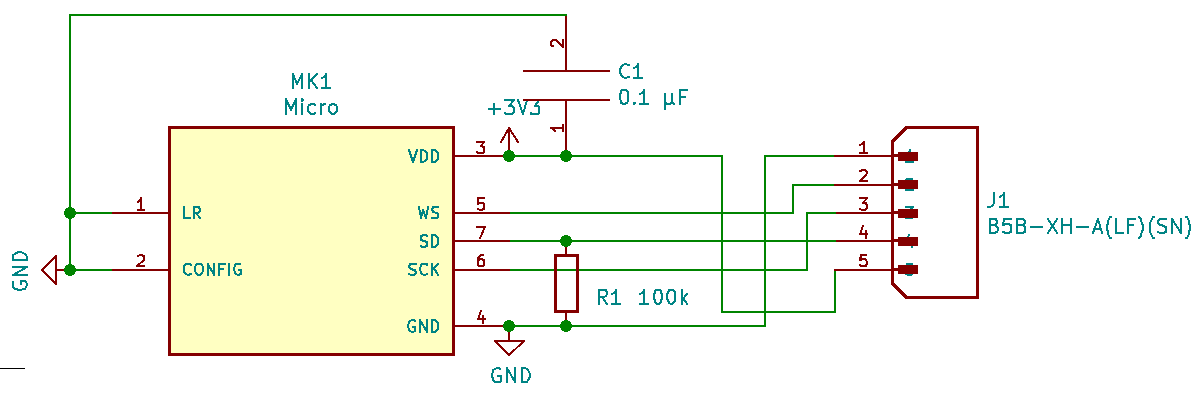
\includegraphics[width=1\textwidth,height=1\textheight,keepaspectratio]{figs/Schematic.PNG}
    	\caption{microphone PCB schematic}\label{fig:radiation}
    \end{figure}
    
    \begin{figure}[hb]\centering
         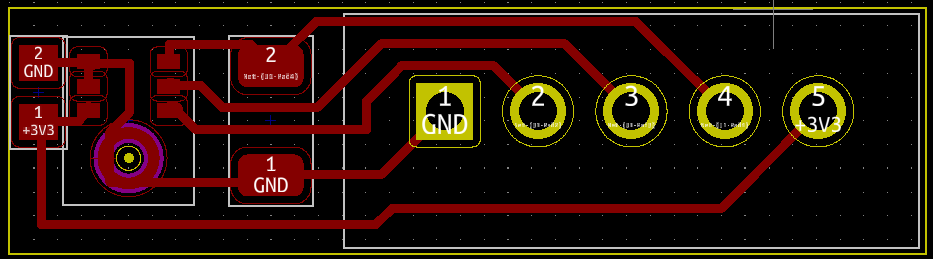
\includegraphics[width=1\textwidth,height=1\textheight,keepaspectratio]{figs/PCB_2Dmodel.PNG}
    	\caption{microphone PCB 2D model}\label{fig:radiation}
    \end{figure}
    
    \begin{figure}[hb]\centering
         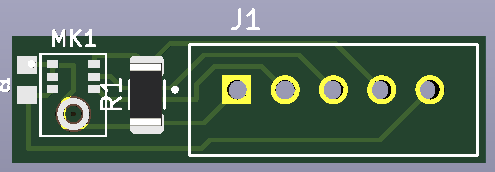
\includegraphics[width=1\textwidth,height=1\textheight,keepaspectratio]{figs/PCB_3Dmodel.PNG}
    	\caption{microphone PCB 3D model}\label{fig:radiation}
    \end{figure}
    
